%!TEX root = ../thesis.tex

\newcommand{\vrms}{\text{v}_\text{n}^\text{rms}}
\newcommand{\vsq}{\overline{\text{v}_\text{n}^2}}
\newcommand{\vn}{\text{v}_\text{n}}
\newcommand{\vin}{\text{v}_\text{in}}
\newcommand{\vout}{\text{v}_\text{out}}
\newcommand{\Sin}{\text{S}_{\vn}^\text{in}}
\newcommand{\Sout}{\text{S}_{\vn}^\text{out}}
\newcommand{\Svn}{\text{S}_{\vn}}


\chapter{Noise characterization}
\label{ch:noise}
% TODO: Left to find out:
% Is the power to V_in conversion correct?

When performing measurements one is faced with the reality that no component is ideal. When a signal passes through the different parts of a set-up, noise is constantly being added. Noise is the term given for all the random fluctuations that are added to the signal. These fluctuations are the cumulative result of several noise source contributions.

Thermal noise is one of the most common sources of noise. It is the result of the random thermal fluctuations of electrons. It is an example of frequency-independent noise, also known as white noise. Noise sources can also be frequency-dependent, such as TLS, as discussed in Ch.~\ref{part:DRIE}. This is an example of $1/f$-noise: the amount of noise added increases with decreasing frequency. In fact, truly frequency-independent noise does not exist, as even white noise has been observed to decrease at extremely high frequencies (\SI{\sim e15}{\hertz}). At these frequencies a quantum correction needs to be added \cite[p50]{vasilescu2006electronic}.

When performing measurements one important question to ask is how much noise is being contributed to the signal. In this chapter a model is presented for the general set-up used for measuring superconducting resonators and qubits. Using this model it is possible to characterize the amount of noise by determining its associated noise temperature. Finally, this model is applied to the set-up used to characterize the resonators presented in Ch.~\ref{part:DRIE}.

\section{Characterizing noise}

\subsection{Circuit representations}


\begin{figure}[h]
    \centering
    \begin{subfigure}[b]{.43\textwidth}
        \includegraphics[width=\textwidth]{Figures/Noise/thevenin.png}%\figureinset{(a)}{2.55}{1.5}
        \caption{Th\'evenin representation}
        \label{fig:thevenin}
    \end{subfigure}
    \begin{subfigure}[b]{.49\textwidth}
        \includegraphics[width=\textwidth]{Figures/Noise/norton.png}%\figureinset{(b)}{2.55}{1.5}
        \caption{Norton representation}
        \label{fig:norton}
    \end{subfigure}
    \caption{Two equivalent representations of a system containing noise. Panel~\textbf{(a)} shows the Th\'evenin representation, in which a noiseless voltage source is connected in series with a noise voltage source. Panel~\textbf{(b)} shows the Norton representation, in which a noiseless current source is connected in parallel with a noise current source.}
\end{figure}

There are two circuit representations in which we can depict a system with a noise contribution: The Th\'evenin representation, and the Norton representation. In the Th\'evenin representation we can model the system as a voltage source, and the noise added to the system is a noise voltage source connected in series. In the Norton representation the system is a current source and the noise added is a noise current source connected in parallel to the current source. These two representations are identical and can be converted to each other. In this section we will adopt the Thev\'enin representation, and so the signal will be a voltage source combined in series with a noise voltage source.

Assuming the signal to be at a fixed frequency $\omega$ and amplitude $A$, the combined voltage $v(t)$ is then given by:

\begin{equation}
    \text{v}(t) = \text{v}_\text{signal}(t) + \text{v}_\text{noise}(t) = A \cos{\omega t} + \vn(t)
\end{equation}

Note that the mean value of the noise voltage $\overline{\vn}$ is equal to zero. The amount of noise can be quantified by the root-mean square noise voltage $\vrms$:
\begin{equation}
    \vrms = \sqrt{\overline{\text{v}^2} - \overline{\text{v}}^2} = \sqrt{\vsq}
    \label{eqn:v_rms}
\end{equation}

\subsection{Noise power spectral density}

One way of quantifying the noise of the system is through the noise power spectral density $S(f)$, which is the distribution of noise power per unit bandwidth as a function of frequency. For the Th\'evenin representation, the noise spectral density is defined in terms of voltage. When the only noise in the system is white noise, the spectral density is independent of frequency. It is then given by:

\begin{equation}
    S = \frac{\vsq}{\Delta f}
    \tagaddtext{[\si[per-mode=symbol]{\volt \squared \per \hertz}]}
    \label{eqn:noise spectral density definition}
\end{equation}

In this equation $\Delta f$ is the noise bandwidth. This is the bandwidth over which the noise is measured.

\newpage
\section{The model}

\begin{figure}
    \centering
    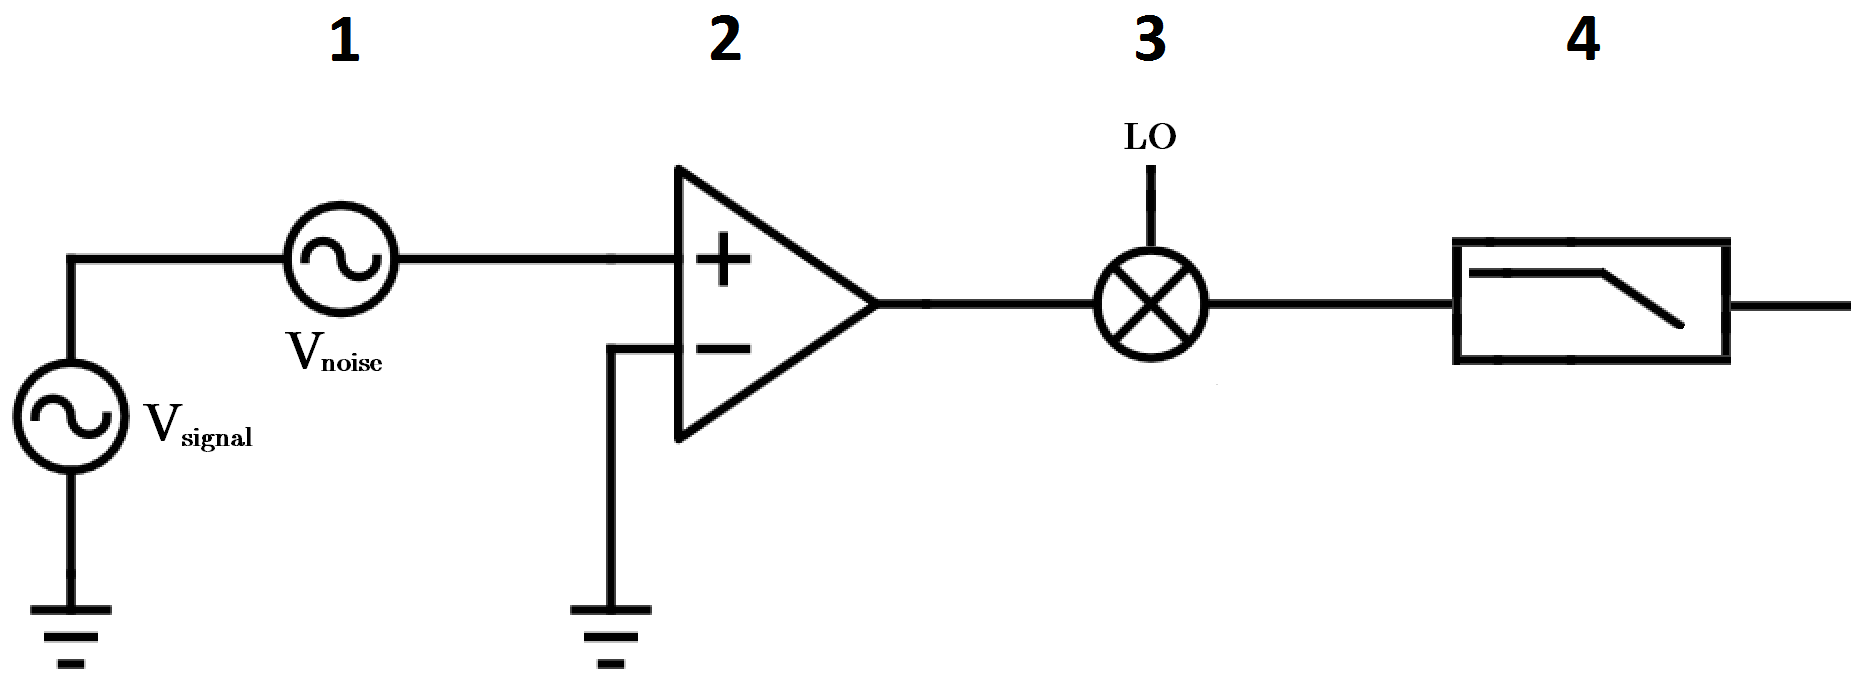
\includegraphics[width=.8\textwidth]{Figures/Noise/Noise model.png}
    \caption{Schematic representation of the measurement set-up including a noise source.}
    \label{fig:noise model}
\end{figure}


As shown in the schematic in Fig.~\ref{fig:noise model}, we can model our set-up as a combination of four elements:

\begin{enumerate}
    \item A noise source.
    \item An amplifier to amplify the weak signal exiting the fridge.
    \item A mixer to downconvert the signal.
    \item A low-pass filter to remove unwanted high-frequency signal.
\end{enumerate}



\subsection{Noise source}

Using the Th\'evenin model, we can approximate the components up to the first amplifier in the fridge as a voltage source, with a noise voltage source connected in series.

We can include the noise added by the amplifier in the noise voltage source, in which case we assume the amplifier to be ideal. Furthermore, we assume the signal to be amplified sufficiently, such that the mixer and low-pass filter add a negligible amount of noise. We also ignore effect such as mixer leakage. With these assumptions all of the noise is originated from the noise voltage source.

We can associate an effective noise temperature to the noise voltage source. The noise temperature is defined as the temperature at which a resistor would produce an equal amount of noise. Note that, since we are comparing the system to a resistor, the noise needs to have an (approximately) white spectrum.

According to Nyquist's theorem \cite[p47]{vasilescu2006electronic}, if the system experiences white noise, and is in thermal equilibrium, the root-mean square noise voltage $\vrms$ is given by:

\begin{equation}
    \vrms = \sqrt{\vsq} = 4 k_B T R \Delta f
    \label{eqn:noise rms voltage}
\end{equation}

In this equation $\Delta f$ is the bandwidth over which the noise is integrated, $k_B$ is the Boltzmann constant, $T$ is the noise temperature of the noise source, and $R$ is the impedance of the system. We see that the noise added depends linearly on the bandwidth over which is integrated.

Combining Eqs.~\ref{eqn:noise spectral density definition} and~\ref{eqn:noise rms voltage}, the noise power spectral density $S_{\vn}$ can be rewritten as:

\begin{equation}
S = \frac{\vsq}{\Delta f} = 4 k_B T R
\end{equation}





\subsection{Amplification}
During the amplification stage both the signal and the noise is amplified by the same amount. This amount of amplification is determined by the gain $G$, which is defined as the ratio between the output voltage and the input voltage:

\begin{equation}
    G = \frac{\text{v}_\text{out}}{\text{v}_\text{in}}
    \label{eqn:gain}
\end{equation}

According to the maximum power transfer theorem, the maximum power transfer between a source and load occurs when the impedances of source and load are matched, in which case half of the power is transferred. From this it follows that in the amplification process half of the signal is dissipated. However, as $G$ is defined as the ratio between $\text{v}_\text{out}$ and $\text{v}_\text{in}$ (see Eq.~\ref{eqn:gain}), the factor $\frac{1}{2}$ is included in $G$.

During amplification not only the signal is amplified with gain G: the noise is amplified by the same amount. Defining the noise power spectral density before amplification as $S^\text{in}$, and after amplification as $S^\text{out}$, the following relation holds:

\begin{equation}
    S^\text{out} = G^2\; S^\text{in} = G^2 4 k_B T R
    \label{eqn:noise power spectral density amplification}
\end{equation}

Note that in Eq.~\ref{eqn:noise power spectral density amplification}, the gain $G$ is squared. This is due to the fact that the noise power spectral density depends quadratically on the root-mean square noise voltage (Eq.~\ref{eqn:noise spectral density definition}).

In our actual set-up the amplification occurs in multiple stages. Aside from amplifying the signal and its noise, at each stage additional noise, originating from the amplifier itself, is added as well. This added noise is then also amplified in the next amplification stage.   Therefore it is always best to have the amplifier with highest gain and lowest noise temperature as the first amplifier in the chain. For more information see Friis formula \cite[p103]{vasilescu2006electronic}.



\subsection{Downconversion}

After amplification the frequency $\omega$ of the signal is still in the GHz range. In homodyne or heterodyne detection the signal is downconverted to DC (homodyne) or to a lower frequency (heterodyne), such that it can be measured more easily. To downconvert the signal, it is mixed in a mixer with a local oscillator (LO) signal having the same frequency $\omega$ (homodyne) or a slightly higher frequency $\omega + \Delta \omega$ (heterodyne). The mixer effectively multiplies the two signals. If the signal exiting the amplifier is given by $\text{v}(t) = A\cos \omega t$, then, ignoring a possible phase difference, the signal at the output of the mixer is given by:

\begin{align}
    \text{v}(t) \cdot \cos{\omega t}& = A \cos{\omega t} \cdot \cos{(\omega + \Delta \omega ) t} \notag\\
        & = \frac{1}{2} A \left[\cos{(2\omega + \Delta \omega)t} + \cos{\Delta \omega t}\right]
        \label{eqn:mixer}
\end{align}

As can be seen from Eq.~\ref{eqn:mixer}, the output signal contains both the sum and the difference of the two signals. However, as the sum of both frequencies is in the GHz range, it can be filtered out using a low-pass filter, leaving only the downconverted signal, which is the result of the difference between the two frequencies. Note that the amplitude of the signal is reduced by a factor two. The noise amplitude is also reduced by a factor 2. Furthermore, in the case of a homodyne set-up, the difference signal is simply a DC signal ($\Delta \omega = 0$), while in the case of heterodyne the signal still contains a slow frequency $\Delta \omega$. For simplification we assume our set-up to be a homodyne set-up, although the result is similar in the case of a heterodyne set-up.

\subsection{Low-pass filtering}

In the case of homodyne detection the signal at the frequency of interest is downconverted to DC. However, the signal at other frequencies have not disappeared; in the mixer these have also shifted in frequency. Since the signal of interest is at DC, a low-pass filter can be used to filter out signal above a certain frequency.

The frequency above which a low-pass filter will filter out the signal is defined by its cut-off frequency $f_\text{c}$. The cut-off frequency $f_\text{c}$ is the frequency at which the signal is attenuated by \SI{3}{\decibel}. For first-order low-pass filters the noise bandwidth $\Delta f$ is related to the filter cut-off frequency $f_\text{c}$ by \cite[p81]{vasilescu2006electronic}:

\begin{equation}
    \Delta f = \frac{\pi}{2} f_\text{c}
    \label{eqn:noisebandwidth}
\end{equation}

\section{Noise temperature}

In the previous sections the influence of each of the components on the signal and on the noise has been analyzed. Using this information it is possible to determine the signal-to-noise ratio (SNR), which is the ratio between the average power of the signal and the average power of the noise. The SNR is a measure for how well a signal can be separated from the noise, and is given by:

\begin{align}
    \text{SNR} = \frac{\overline{\vout}^2}{\vsq} = & \frac{1/4 \;G^2 \; \overline{\vin}^2}{ \Sout \; \Delta f}\notag\\
        = & \frac{1/4 \; G^2 \; \overline{\vin}^2}{G^2 \; \Sin \;\frac{\pi}{2}\;f_\text{c}}\notag\\
        = & \frac{\overline{\vin}^2}{2 \; \pi \; k_B \; T \; R \; f_\text{c}}
    \label{eqn:SNR}
\end{align}

% TODO: factor 1/4 for both signal and noise?
Note that the factor $1/4$ is because the amplitude is lowered by a factor of $2$ due to mixing. Equation~\ref{eqn:SNR} can be rewritten such that we have an expression for the noise temperature of the system:

\begin{equation}
    T =\frac{\overline{\vin}^2}{2 \; \pi \; k_B \; R \; f_\text{c} \; \text{SNR}}
    \label{eqn:noise temperature}
\end{equation}


\section{Results}
\label{sec:noise_results}
\begin{figure}[h]
    \centering
    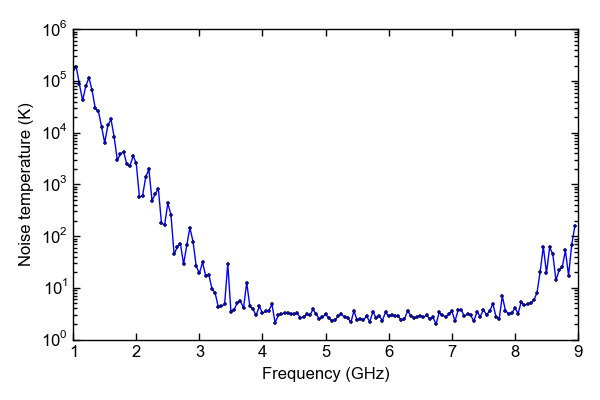
\includegraphics[width = .7 \linewidth]{Figures/Noise/noise_temperature_versus_power.png}
    \caption{Noise temperature versus frequency. The noise temperature has been calculated for $160$ frequencies in the range \SIrange{1}{9}{\giga \hertz}. For each frequency $2001$ points were measured, from which the signal, noise, SNR, and noise temperature was determined. Measurements were performed at an input power of \SI{-113}{\dBm} and an IF bandwidth of $\Delta f = $\SI{300}{\hertz}.}
    \label{fig:Noise temperature}
\end{figure}

Using the Rhode \& Schwarz ZVM vector network analyzer, The transmission has been measured for $160$ equidistant frequencies in the range \SIrange{1}{9}{\giga \hertz}. For each frequency a total of $2001$ points was measured with an IF bandwidth $\Delta f = $ \SI{300}{\hertz}. From these measurements the signal-to-noise ratio has been determined for each frequency. With knowledge of the SNR, the noise temperature has then been determined as a function of frequency using Eq.~\ref{eqn:noise temperature} . The result is shown in Fig.~\ref{fig:Noise temperature}.

From Fig.~\ref{fig:Noise temperature} it is clear that the noise temperature is highly temperature-dependent. In the frequency range \SIrange{4}{8}{\giga \hertz} the noise temperature is quite low, never reaching above \SI{10}{\kelvin}. This is exactly the bandwidth of the cryogenic low-noise amplifier by Low Noise Factory, which is the first amplifier in the amplification chain. From the specifications of the amplifier, the noise temperature of the amplifier has been calculated at an ambient temperature of \SI{8}{\kelvin}, and equals roughly \SI{4}{\kelvin} for the entire bandwidth. Comparing the amplifier specifications with Fig.~\ref{fig:Noise temperature}, it is likely that in the frequency range \SIrange{4}{8}{\giga \hertz} the first amplifier is the component contributing most to the total noise temperature.

Outside the \SIrange{4}{8}{\giga \hertz} frequency band, however, the noise temperature rapidly increases. This is partly due to the frequency lying outside of the bandwidth of the amplifier, in which case the amplification will be lower. However, this is not an adequate explanation for the fact that the noise temperature increases to several hundred thousand Kelvin. The reason for this unrealistic noise temperature is that in our model we did not take into account the noise added by components after the amplifier. While the gain of the amplifier decreases outside its bandwidth, the components after the amplification will still add the same amount of noise. When the gain decreases by a significant amount, the relative contribution of these post-amplification noise sources will increase. Furthermore the assumption that the noise spectrum is white is no longer correct at low frequencies, where $1/f$ noise starts to contribute.

\begin{figure}[h]
    \centering
    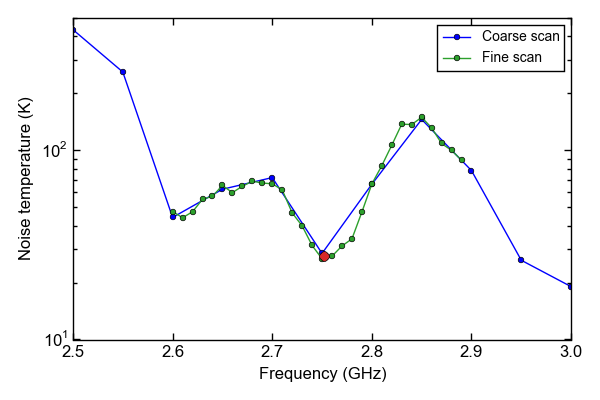
\includegraphics[width = .6\linewidth]{Figures/Noise/noise_temperature_versus_power_detailed.png}
    \caption{Detailed scan of noise temperature versus frequency in the range \SIrange{2.6}{2.9}{\giga \hertz}. The resonator with $f_0 = $\SI{2.75}{\giga \hertz} (red dot) seems to reside at a local minimum of the noise temperature.}
    \label{fig:noise temperature 2GHz}
\end{figure}

From Fig.~\ref{fig:Noise temperature} it can be seen that the noise temperature can vary by a large amount between consecutive points. To determine whether this variation is due to a large uncertainty, or due to the noise temperature actually fluctuating strongly with varying frequency, a more detailed scan has been performed in the frequency region \SIrange{2.6}{2.9}{\giga \hertz}, in which one resonator has a resonance frequency. The result is shown in Fig.~\ref{fig:noise temperature 2GHz}. As the curve of the detailed scan follows the curve of the coarse scan pretty closely, it can be concluded that the noise temperature of the system in fact fluctuates quite strongly with varying frequency.

Another point of interest is that the resonance frequency of the resonator lies near the local minimum of the noise temperature in that region. This is quite a stroke of luck, as a slightly higher or lower frequency would have resulted in a much higher noise temperature.



\section{Conclusion and future work}

The noise temperature gives us an estimate of the noise added to the system. It has been shown that the noise temperature can fluctuate strongly with varying frequency. In the model used to estimate the noise temperature it has been shown that outside the bandwidth of the amplifier the model breaks down. At this point the noise added by the components after the amplification, and indeed even the amplifiers themselves, needs to be taken into account to obtain accurate estimates of the noise temperature.

However, even outside of the bandwidth of the amplifier, there are frequency regions in which the noise temperature may still be acceptable. It is therefore a good idea to initially perform measurements of the noise temperature of the set-up. This will give an indication of the signal-to-noise ratio, from which accurate estimates can be made as to what the amount of measurement time is needed to obtain a desired SNR.

The noise temperature measurements were performed using the Rhode \& Schwarz ZVM vector network analyzer. It would be interesting to see how other measurement set-ups would compare to the vector network analyzer. One interesting candidate would be a heterodyne detector. However, as the vector network analyzer can also measure phase, a fair comparison would also require the heterodyne detector to be able to measure the phase. This heterodyne detector is currently being set up, and will hopefully soon yield interesting results.

Aside from only comparing the noise temperature, other properties are also important when comparing two set-ups. One of these is the duty cycle, which is the percentage of time acually spent measuring. For the vector network analyser the duty cycle seems to be around $50\%$, provided that a single measurement sweep takes at least a few seconds. Other set-ups may therefore offer an improvement in the duty cycle. Furthermore, properties such as phase stability and uncertainty would also be interesting to compare.

Another interesting measurement would be to see if the noise temperature as a function of frequency remains the same in future cooldowns, and for different samples.

